\icode{E-MI-CA-L3-261026-001}
一个质量\(m =\)	\,\qty{0.5}{kg}的小物块（可以看成质点），以\(v_0 =\) \,\qty{2}{m/s}的初速度在平行斜面向上的拉力\(F =\) \,\qty{6}{N}作用下沿斜面向上做匀加速运动，经\(t =\) \,\qty{2}{s}的时间物块由\(A\)点运动到\(B\)点，\(A\)、\(B\)之间的距离\(L =\) \,\qty{8}{m}，已知斜面倾角\(\theta =\) \,\qty{37}{\degree}，重力加速度\(g\)取\qty{10}{m/s^2}，\(\sin\) \,\qty{37}{\degree}\( = 0.6\)，\(\cos\) \,\qty{37}{\degree}\( = 0.8\)。求：
\begin{enumerate}
	\item 物块加速度\(a\)的大小；
	\item 物块与斜面之间的动摩擦因数\(\mu\)；
	\item 若拉力\(F\)的大小和方向可调节，如图所示，为保持原加速度不变，\(F\)的最小值是多少。
\end{enumerate}

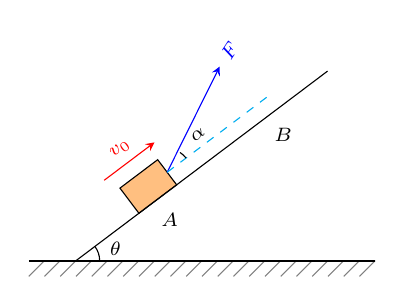
\begin{tikzpicture}[>=stealth,font=\scriptsize]
	\begin{scope}[rotate=37]
		\draw[fill=orange!50] (1,0) rectangle(1.6,.4);
		\draw[->,blue] (1.6,.2)--++(26.57:1.5)node[rotate=57,right]{\(F\)};
		\draw[dashed,cyan] (1.6,.2)--++(1.6,0);
		\draw (0,0)--(4,0);
		\draw[->,red] (.9,.6)--node[above,rotate=37]{\(v_0\)}(1.7,.6);
		\draw (1.9,.2) arc(0:20:.3);
        \node at(2.2,.35)[rotate=37]{\(\alpha\)};
	\end{scope}
	\foreach \x in {-.6,-.4,...,3.8}
		\draw[gray] (\x,-.2)--++(.2,.2);
	\draw[thick] (-.6,0)--(3.8,0);
	\draw (.3,0) arc(0:37:.3);
	\node at(.5,.15){\(\theta\)};
	\node at(37:1.2)[below right]{\(A\)};
	\node at(37:3)[below right]{\(B\)};
\end{tikzpicture}
\begin{answer}
    （1）\(a =\)\,\qty{2}{m/s^2}（2）\(\mu = 0.5\)（3）\(F_{\min} = \frac{12 \sqrt{5}}{5}\) \qty{}{N}\qquad 提示：物块有沿斜面向上的加速度\(a\)，可以添加一个大小为\(ma\)方向沿斜面向下的力，使物块处于平衡状态。将摩擦力与垂直斜面的支持力合成为全反力，该力的方向不变；将\(ma\)与重力\(mg\)合成，合力的大小与方向都不变，如下图所示，当\(F\)与全反力垂直时最小

    \begin{tikzpicture}[>=stealth,font=\scriptsize]
        \draw[dashed,cyan] (37:-2)--(37:2) (-53:1.5)--(127:1.5);
        \draw[->] (0,0)--(0,-2)node[below right]{\(mg\)};
        \draw[->,teal] (0,0)--(37:-.4)node[above left]{\(ma\)};
        \draw[dashed,gray] (37:-.4)--++(0,-2)coordinate(f1)--++(37:2.4)coordinate(f2)--(0,0);
        \draw[->,teal] (0,0)--(f1);
        \draw[->,blue] (0,0)--++($1*($(0,0)-(f2)$)$)node[left]{\(F_{\text{全反力}}\)};
        \draw[->,magenta] (f1)--(153.6:-0.18)node[above right]{\(F\)};
    \end{tikzpicture}
\end{answer}